\begin{tikzpicture}[
every node/.style={anchor=north west,inner sep=0pt},
x=1mm, y=1mm,
]
 
\node[draw,text width=260mm] at (0,-5) {
	\begin{tcolorbox}[height=330mm, title=\large{Introduction}]
		The lithosphere consists of the Earth's crust and the uppermost mantle. It forms the tectonic plates that define continents and oceans. Continental drift and collisions of plates create mountain ranges, sedimentary basins and causes earthquakes and volcanism. The lithosphere can move vertically in response to added load or deeper forces. Studies of the lithosphere has a special importance in Antarctic research as it interacts with ice sheets. \\
		
		This project aims to progress our knowledge about the structure and variability of the deep reaches of the Antarctic continental basement. I will use geophysical observations, e.g. \textit{seismic data}, \textit{airborne gravity} and \textit{magnetotelluric data} to create a new model of the Antarctic lithosphere. This will be constrained with the limited rock type observations and \textit{geochronology}.\\ 
		
		In the tectonic history of the Earth, Antarctica appears to have been a hub in the supercontinent Gondwana assembly (c. 570-180 million years ago) and also of central concern for reconstruction of earlier supercontinents. Therefore, constraints from neighbouring continents can help us to better understand Antarctic geology. \cite{Fisher2015,Boger2011}\\
		
		Until recently, Antarctic geophysical data have been scarce, but extended new datasets are available after the field campaigns begun in the International Polar Year of 2007. I will use a variety of techniques to infer the location and extent of significant hidden tectonic domains from these new datasets. 
%		I hope to find out which parts of Antarctica are most buoyant and where the heat supply to the ice sheets from the rock beneath is greatest. This can contribute to better ice sheet models and better understanding of the Earth response to changing climate. 
	\end{tcolorbox}
	};

\node[text width=260mm] at (280,-5) {
	\begin{tcolorbox}[height=330mm, title=\large{Ice and rocks}]
	 The lithosphere of Antarctica is especially crucial for the interaction between the solid Earth and the ice sheet. The weight of the ice pushes the lithosphere down. How it respond to changes in the glaciation depends on the mechanical properties of the lithosphere, its age and composition.  The buoyancy balance of the lithosphere, the ice sheet and the soft material under the lithosphere is called \textit{isostasy}. \\
	 
	 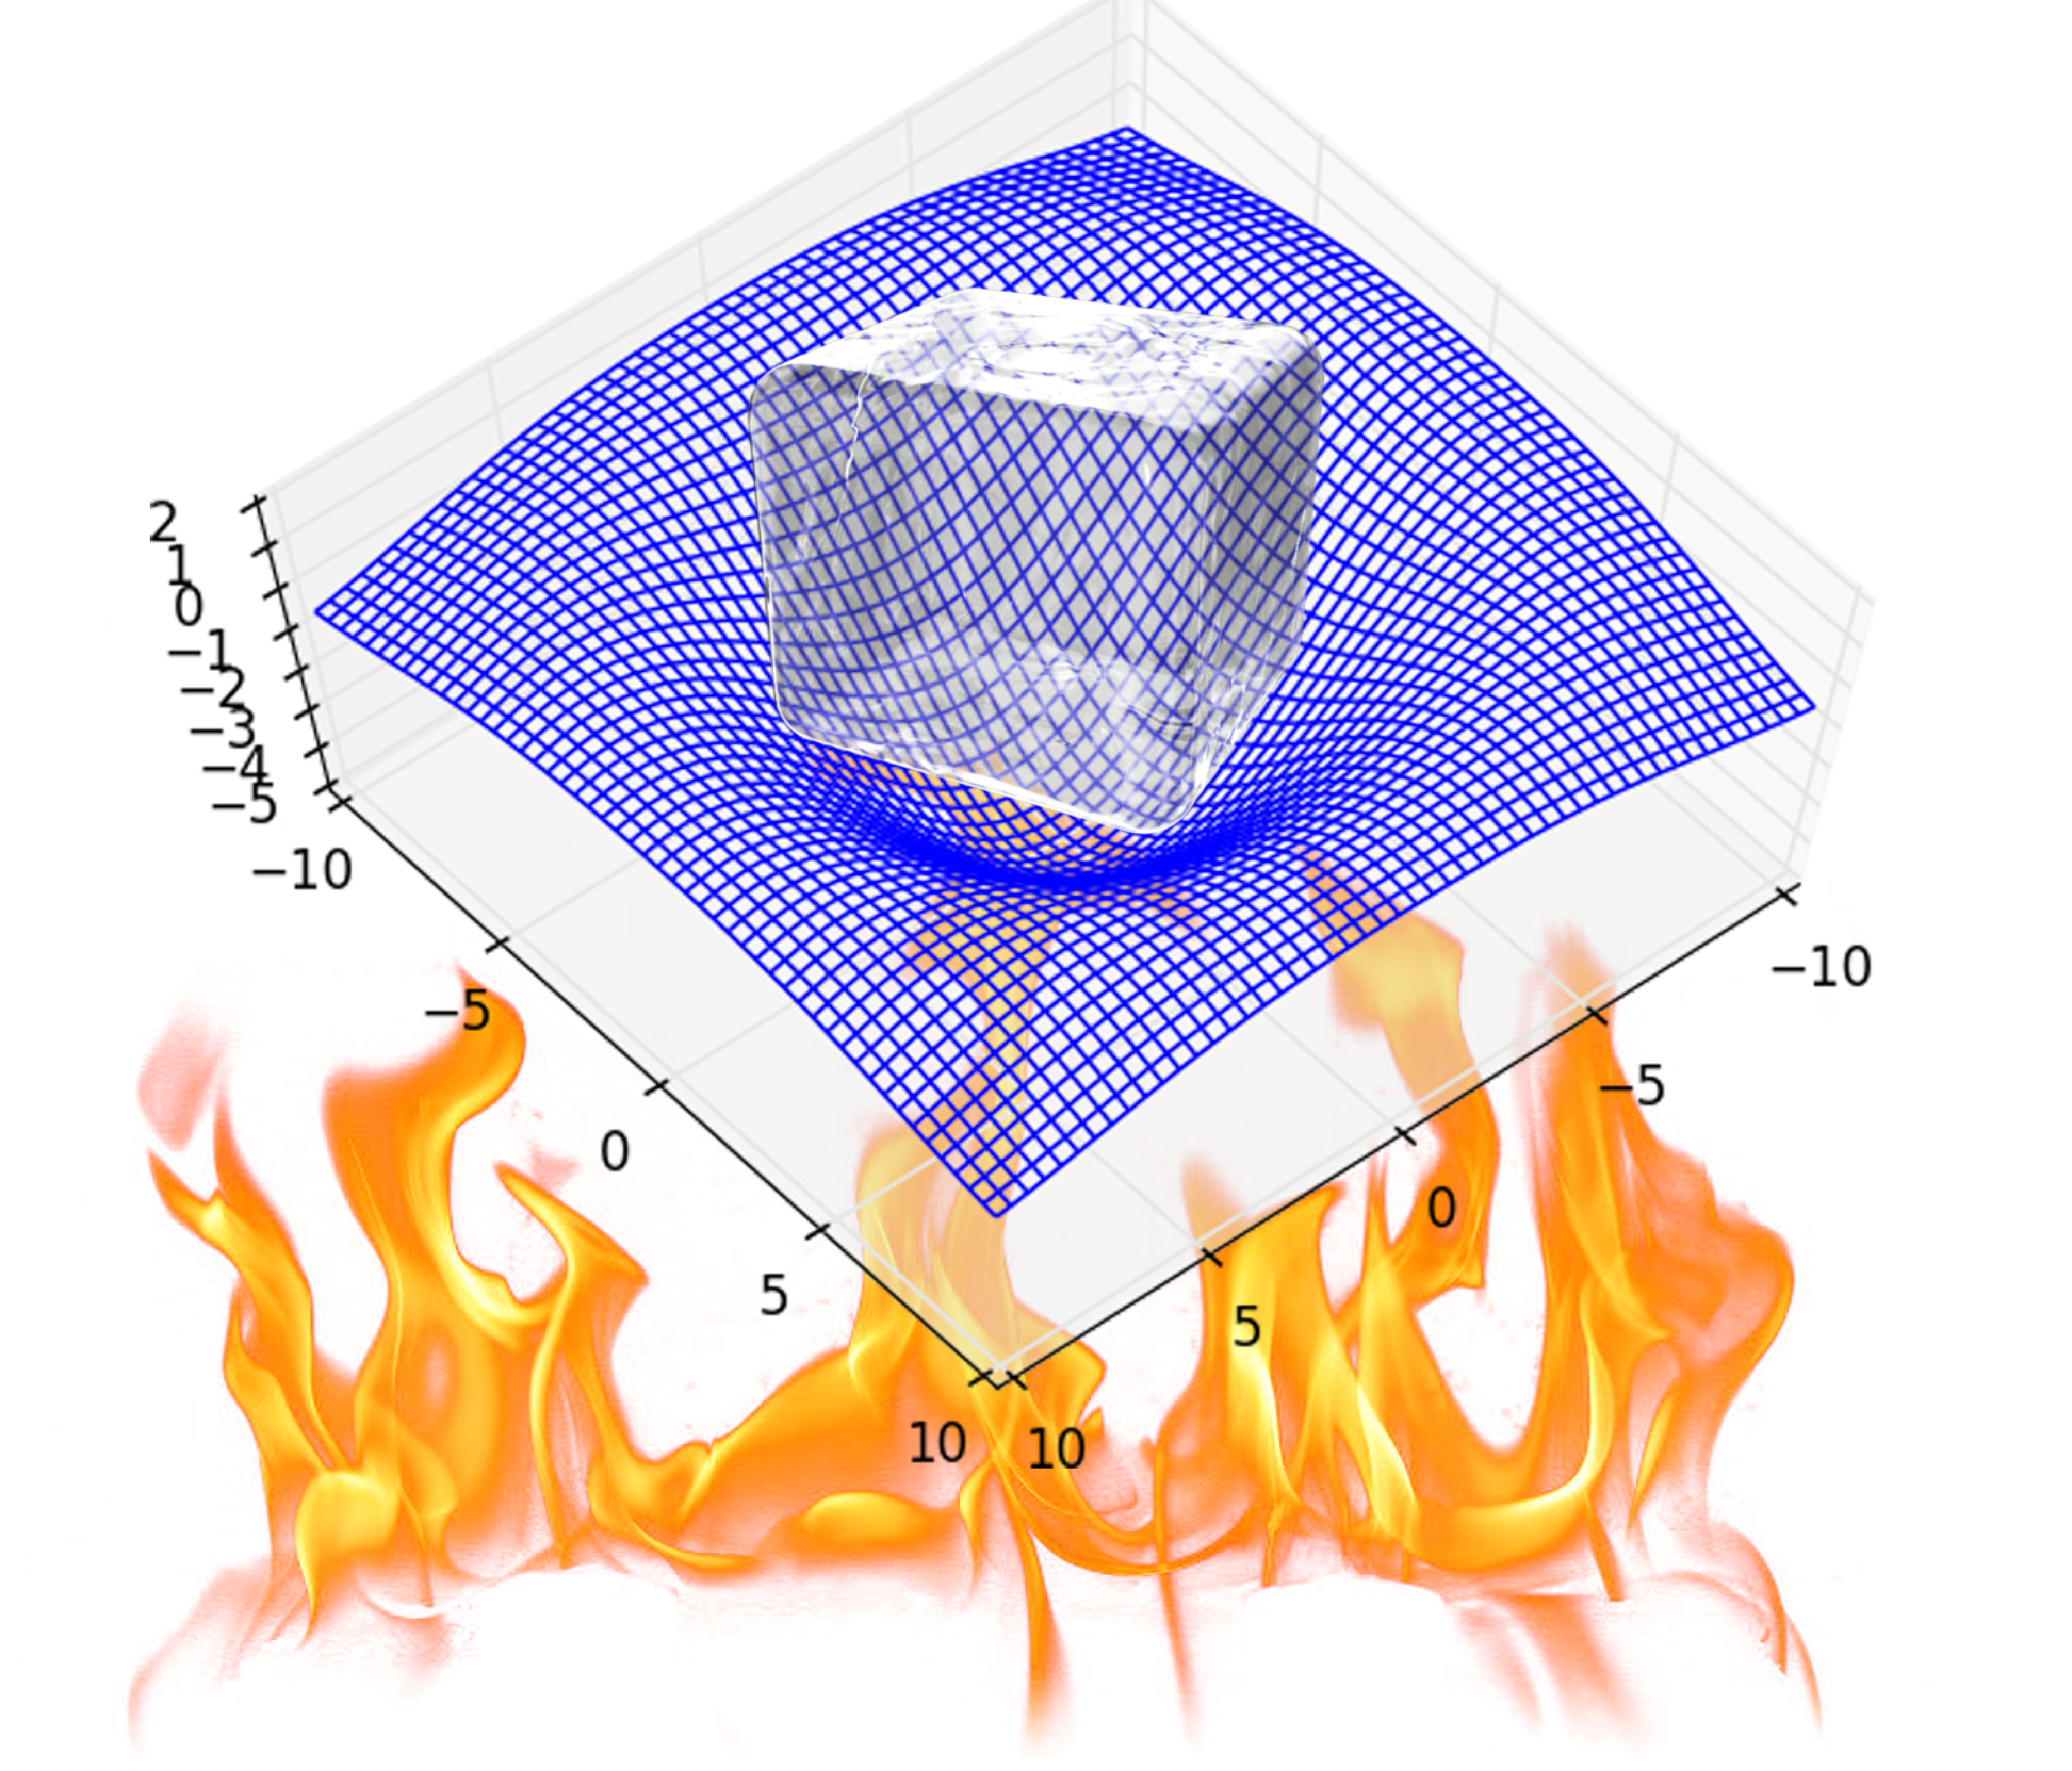
\includegraphics[scale=0.23]{ice_cartoon.pdf}\centering
	 
	 \raggedright
	To estimate how much heat that is transferred to the base of the ice sheets, we need to have a model of the lithosphere. The interior of the Earth is warmer than the surface and the heat is leaving the mantle through the crust and causes basal melting of the ice sheet which in turn leads to formation of sub-glacial lakes, sub-glacial erosion and in some cases instability. The heat originates partly from the formation of the Earth, but the larger fraction, 83\% of the total global heat flow, comes from radioactive decay. 40\% is generated within the shallow crust. The crustal heat production can vary over a large range depending on the geology \cite{Beardsmore2001, Carson2013}. 


	\end{tcolorbox}
};

%C = 410
%%%%%%%%%%%%%%%%%%%%%%%

\node[text width=260mm] at (560,-5) {
	\begin{tcolorbox}[height=330mm, title=\large{Geological maps with colonial borders}]
	The geology of Antarctica is only known from scarce outcrops along the coast and a few mountains in the interior. Therefore, any geological map of Antarctica is a little more than a guesswork. The boundaries between geological terrains are not more justified than colonial borders through a land of unknown cultures. To be able to estimate the heat flux, we need to have a more truthful map of the geological terrains under the ice \cite{Boger2011}. If boundaries remain uncertain, the probabilities should be mapped.
	
	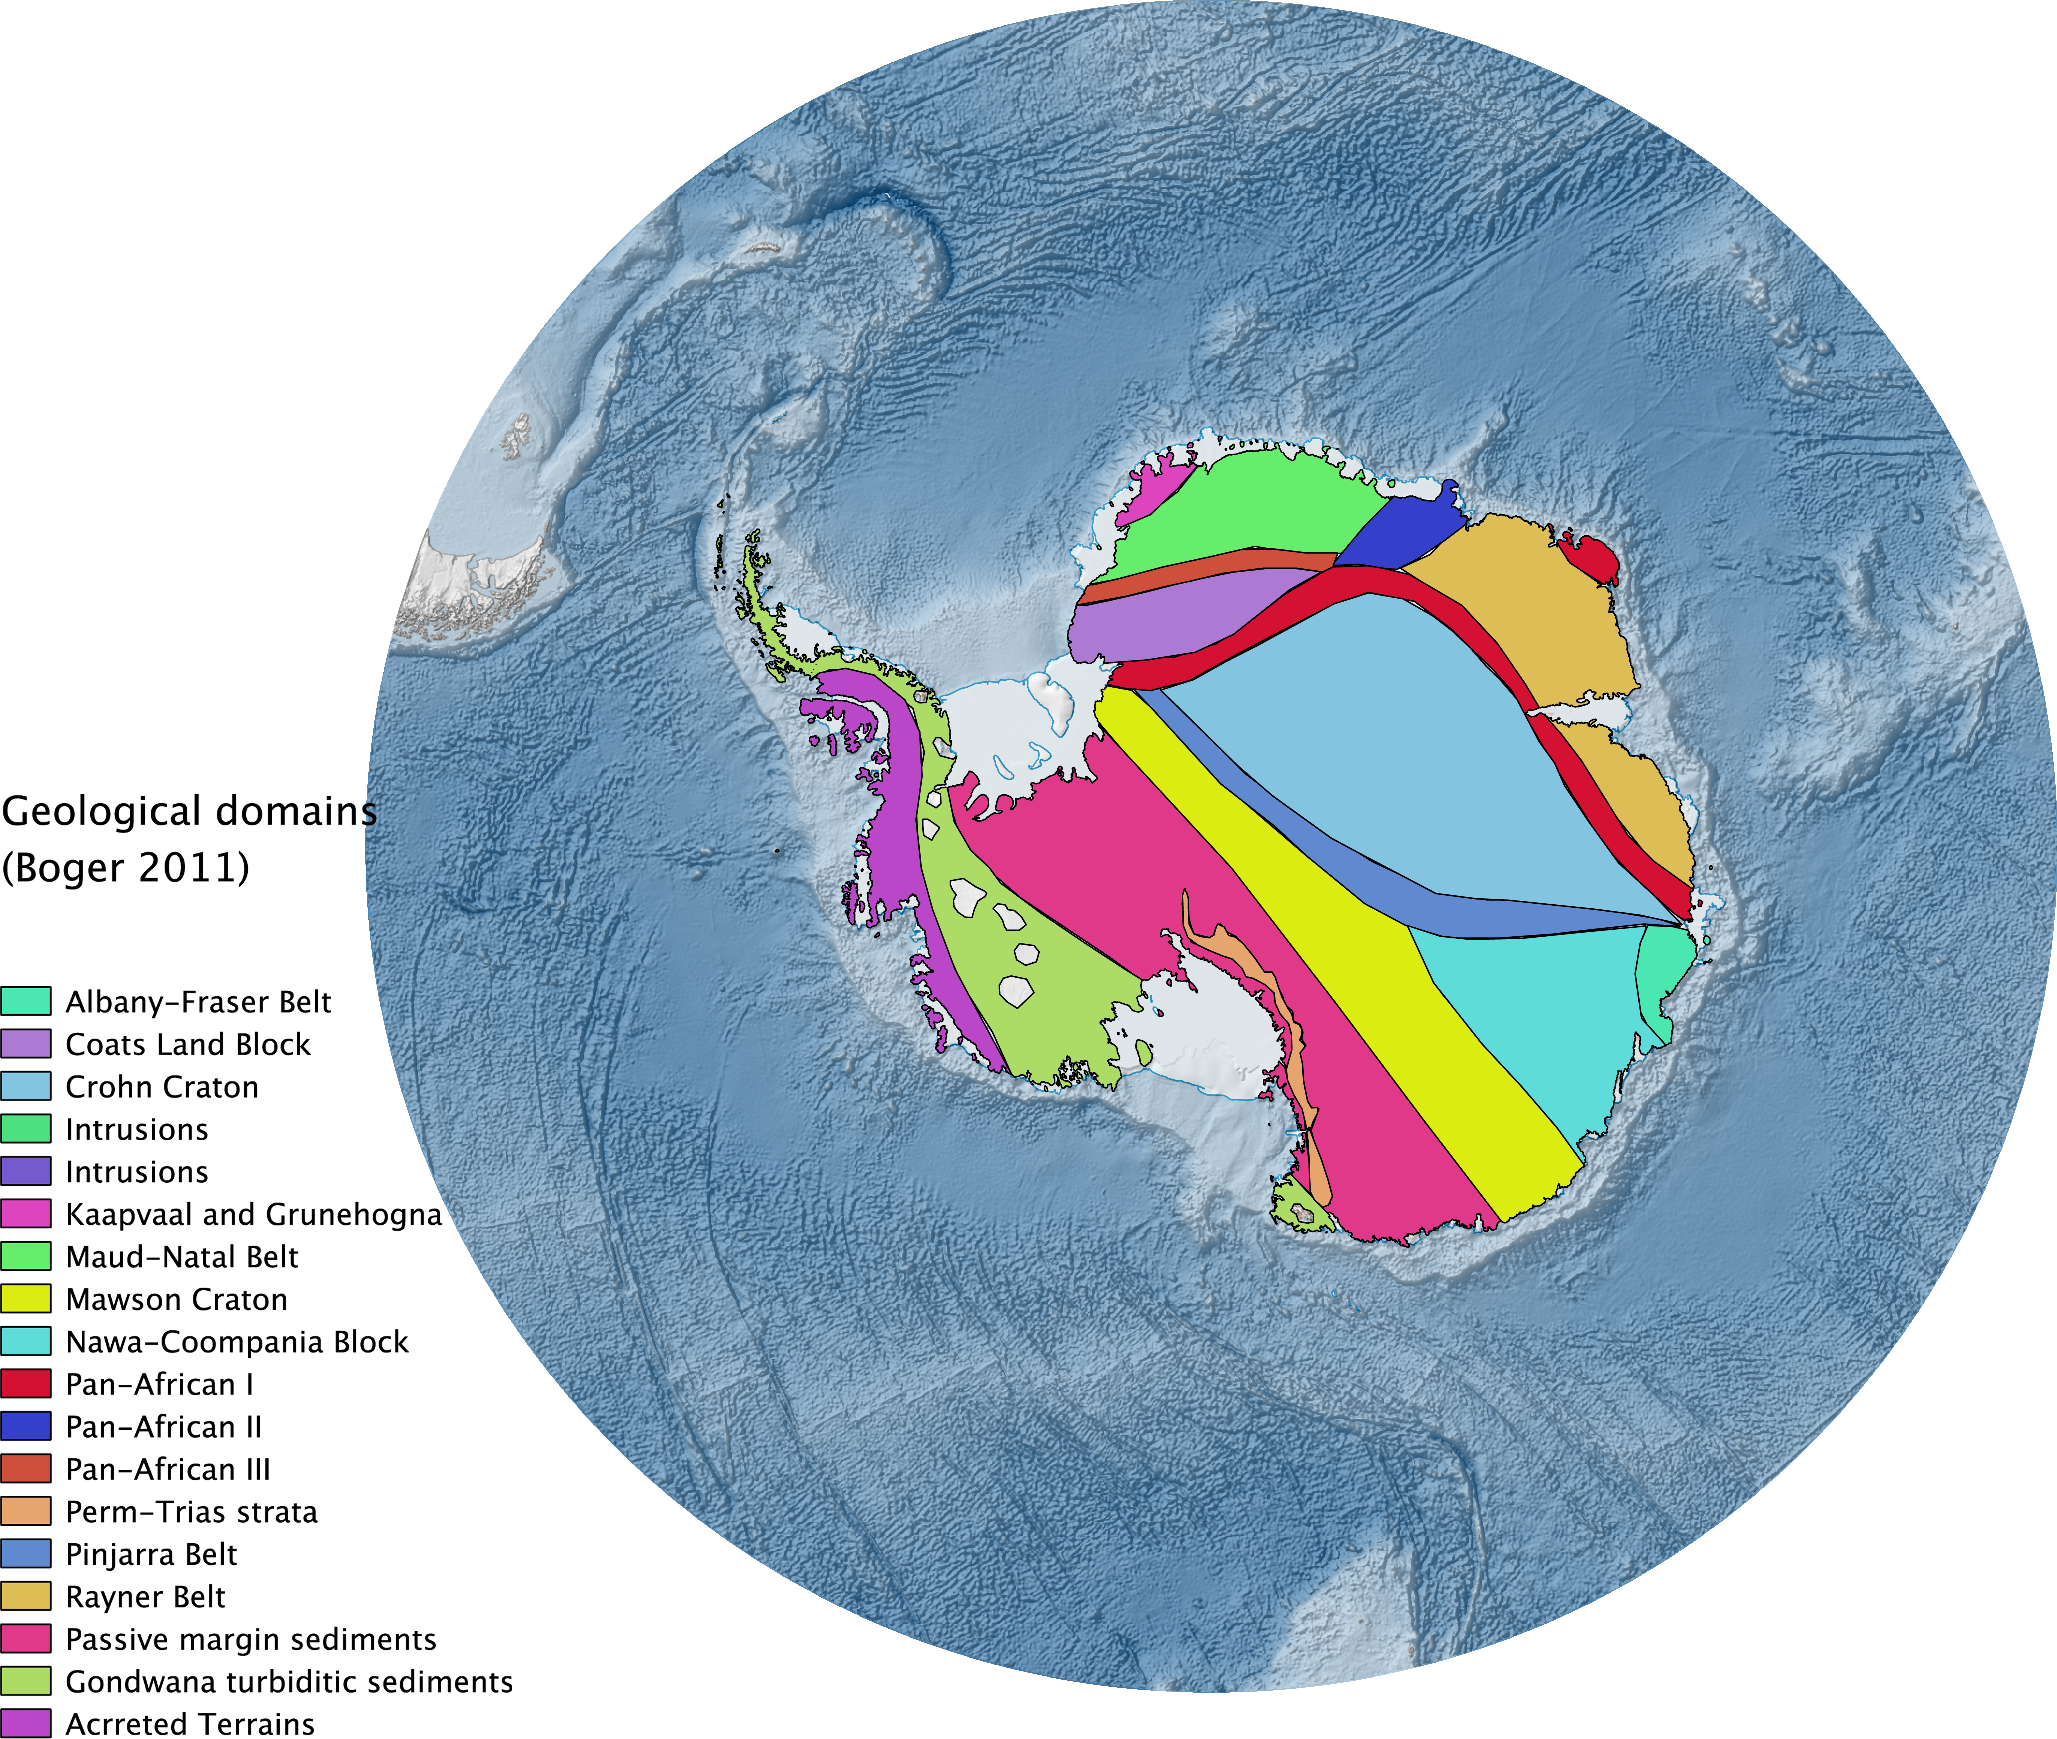
\includegraphics[scale=0.7]{boger_map.pdf}\centering

	\end{tcolorbox}
	
};

\node[text width=253mm] at (0,-344) {
\includegraphics[width=820mm, trim={0 143mm 0 193mm},clip]{photo_ice.jpg}\centering

	
};

%http://sitn.hms.harvard.edu/wp-content/uploads/2016/02/12435253353_15ad92569d_k.jpg


\node[text width=260mm] at (0,-515) {
	\begin{tcolorbox}[height=440mm, title=\large{Estimating the heat flow}]
	
	
	\begin{figure}
	\centering
	\rotatebox{90}{\tiny Data from \citet{An2015}}
	\includegraphics[scale=0.9, trim={0 0 0 0},clip]{An_heat.png}
	\end{figure}	
	
	
	Crustal heat flow in $mW/m^2$ based on seismic velocities and heat transfer functions \cite{An2015}.
	This is our best available method to estimate the heat flow in absence of direct measurements. Hot material generally have a lower velocity and cold material has a higher velocity.  Unfortunately, this kind of models don't agree well with actual direct measurements that locally can be 2-3 times higher. \cite{Fisher2015}
	
	\begin{itemize}
	\item The heat production from within the crust is not well known. This is especially a problem in East Antarctica. Continents that was attached to East Antarctica in Gondwana have high heat production in the crust, e.g. South Australia. \cite{Carson2013} 
	
	\item West Antarctica consists of a complex mosaic of small blocks, volcanism and rifting. To estimate this local variations we need higher resolution and more seismic data. Locally, the East Antarctic litosphere can also be thin. \cite{Reading2006, Boger2011}

	\end{itemize}
	
	\end{tcolorbox}
	
};


\node[text width=260mm] at (280,-515) {
	\begin{tcolorbox}[height=440mm, title=\large{Lithosphere thickness}]
	
	\begin{figure}
		\centering
		\rotatebox{90}{\tiny Data from \citet{An2015}}
		\includegraphics[scale=0.9, trim={0 0 0 0},clip]{An_LAB.png}
	\end{figure}	
	

The depth in $km$ to the boundary between the lithosphere and the \textit{astenosphere} is not unambiguous. It depends on what definition we use for the lithosphere. In this map  thickness is derived from seismic velocities and can be used as constraints for the tectonic regions of Antarctica. Note that East Antarctica is much thicker than West Antarctica, suggesting a different tectonic history. \cite{An2015, Boger2011}

By measuring the time for a seismic event from e.g. an earthquake to a seismometer, we can inverse for the velocity. Unfortunately, in this context, there is not many earthquakes in Antarctica and until recently, it's been very few seismometers. The models have been very course in probably not correct but thanks to the campaigns during the International Polar Year (IPY) 2007-08 we now have more measurements. For high resolution models, even more seismic stations are needed and active seismic sources. 

	\end{tcolorbox}
	
};


\node[text width=260mm] at (560,-515) {
	\begin{tcolorbox}[height=340mm, title=\large{Crustal thickness}]
	
	\begin{figure}
		\centering
		\rotatebox{90}{\tiny Data from \citet{An2015}}
		\includegraphics[scale=0.9, trim={0 0 0 0},clip]{An_CRUST.png}
	\end{figure}
	
	The thickness of the crust in $km$. The crust is  chemically distinct from the mantle, and easier to define. The thickness can be used as correlation between various seismic techniques \cite{An2015}.
	 Different seismic methods don't agree everywhere, e.g \textit{receiver functions} can measure the local crustal thickness with rather good accuracy, \textit{tomography} can be used for larger areas but changes seen in receiver functions are not present in low resolution tomography \cite{Reading2006}. 
	
	\end{tcolorbox}
	
};


\node[text width=260mm] at (560,-860) {
	\begin{tcolorbox}[height=95mm, title=\large{Discussion and conclusion}]
	
A better model of Antarctic lithosphere is needed to create more accurate models for heat flow and isostasy. Present models \cite{An2015} can be improved with a interdisciplinary approach. Constraints from geology and direct measurements can add important parameters. Moreover, a statistical approach to uncertainties can further improve the models. Studies of the Antarctic lithosphere can provide an important missing key.

	\end{tcolorbox}
	
};



\node[text width=260mm] at (0,-960) {
	\begin{tcolorbox}[height=105mm, title=\large{Acknowledgments}]
	\begin{itemize}
	\item \alert{Antarctic Gateway Partnership - Institute for Marine and Antarctic Studies}
	\item Anya Reading, Earth Sciences / IMAS (main supervisor)
	\item Jacqueline Halpin, Earth Sciences / IMAS (supervisor)
	\item Jo Whittaker, IMAS (supervisor)
	
	
	\end{itemize}
	\end{tcolorbox}
};



\node[text width=260mm] at (280,-960) {
	\begin{tcolorbox}[height=105mm, title=\large{References}]
	\nocite{An2015, Boger2011,Williams2016,Beardsmore2001, Aitken2014a, Carson2013, Fisher2015, Reading2006}
	
	\begin{tiny}
	\bibliographystyle{plainnat}
	\bibliography{poster}
	\end{tiny}
	
	\end{tcolorbox}
};



\node[text width=260mm] at (560,-960) {
	\begin{tcolorbox}[height=105mm, title=\large{Contact}]
	
	
	
	\begin{minipage}{0.7\linewidth}   
	Find me here:
				\begin{itemize}
					\item \href{https://www.imas.utas.edu.au}{www.imas.utas.edu.au}
					\item  \href{mailto:tobbe@tripitaka.se}{sven.staal@utas.edu.au}
				\end{itemize}
	\end{minipage}
	\begin{minipage}{0.2\linewidth}
			\includegraphics[width=35mm]{orcid.png}     
	\end{minipage}\\

	\textit{Photo of polar ice and rocks by Andreas Kambanis. Licensed under Creative Commons.}
	\end{tcolorbox}
	
	
};


\end{tikzpicture}


